%This work is licensed under the Creative Commons License Attribution 4.0 International (CC-BY 4.0)
%https://creativecommons.org/licenses/by/4.0/legalcode
\documentclass[rgb]{standalone}
\usepackage{tkz-euclide}
\definecolor{myorange}{hsb}{0.0833, 1, 0.8}
\definecolor{mygreen}{hsb}{0.3333, 1, 0.8}
\definecolor{myblue}{hsb}{0.5833, 1, 0.8}
\definecolor{mymagenta}{hsb}{0.8333, 1, 0.8}
\begin{document}
	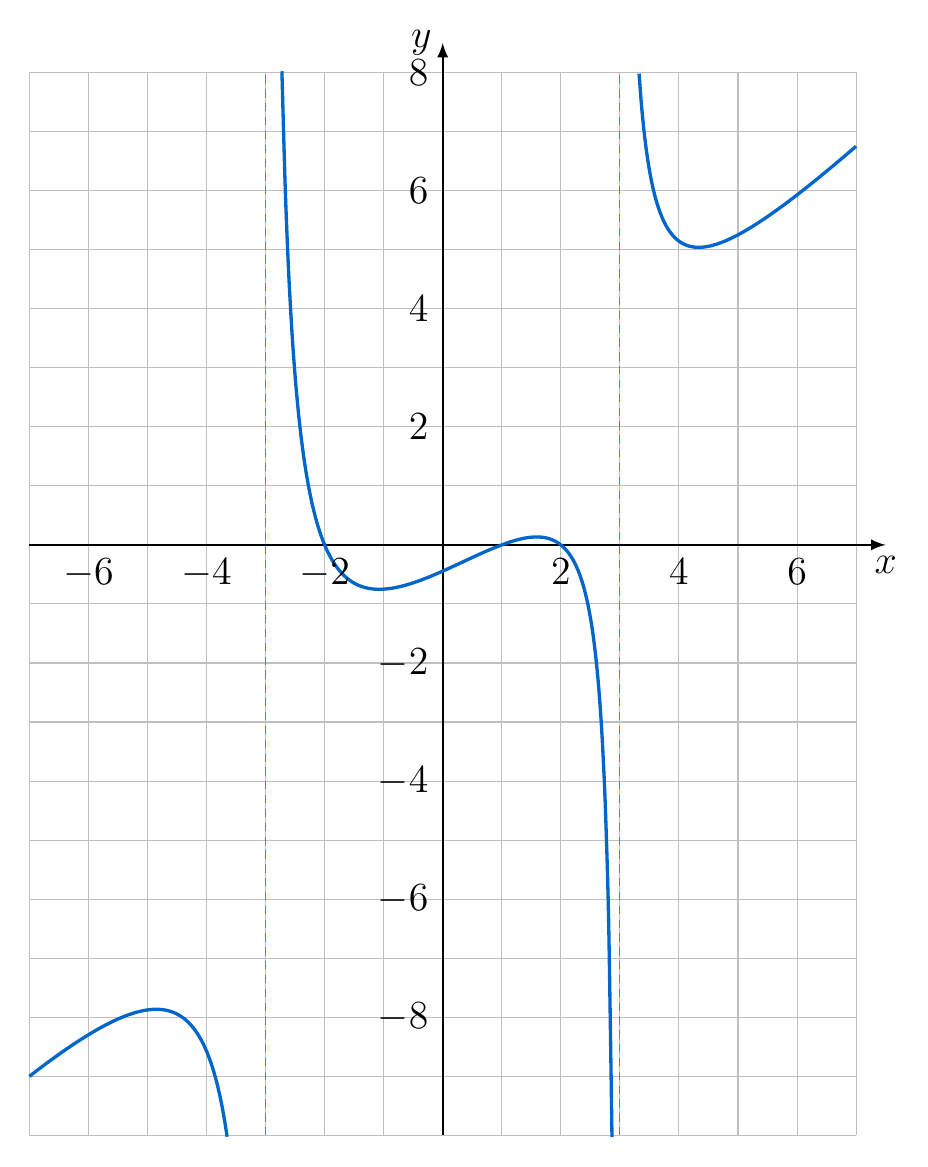
\begin{tikzpicture}[scale=0.75, font=\Large]
		% Coordinate system
		\tkzInit[xmin=-7,xmax=7,ymin=-10,ymax=8]
		\tkzGrid[color=lightgray]
		\tkzDrawX[thick,label=$x$]
		\tkzDrawY[thick,label=$y$]
		% Graphs
		\draw[very thick,myblue,smooth,domain={-7}:{-3.65},samples=100, variable=\x] plot ({\x}, {((\x+2)*(\x-2)*(\x-1)/((\x+3)*(\x-3))});
		\draw[very thick,myblue,smooth,domain={-2.723}:{2.8665},samples=100, variable=\x] plot ({\x}, {((\x+2)*(\x-2)*(\x-1)/((\x+3)*(\x-3))});
        \draw[very thick,myblue,smooth,domain={3.325}:{7},samples=100, variable=\x] plot ({\x}, {((\x+2)*(\x-2)*(\x-1)/((\x+3)*(\x-3))});
        \draw[myorange,,densely dashed] (-3,-10) -- (-3,8);
        \draw[myorange,,densely dashed] (3,-10) -- (3,8);
		% Labels
		\node[below=0.5mm] at (-6,0){$-6$};
	    \node[below=0.5mm] at (-4,0){$-4$};
	    \node[below=0.5mm] at (-2,0){$-2$};
		\node[below=0.5mm] at (2,0){$2$};
		\node[below=0.5mm] at (4,0){$4$};
		\node[below=0.5mm] at (6,0){$6$};
		\node[left=0.5mm] at (0,-8){$-8$};
		\node[left=0.5mm] at (0,-6){$-6$};
		\node[left=0.5mm] at (0,-4){$-4$};
		\node[left=0.5mm] at (0,-2){$-2$};
		\node[left=0.5mm] at (0,2){$2$};
		\node[left=0.5mm] at (0,4){$4$};
		\node[left=0.5mm] at (0,6){$6$};
		\node[left=0.5mm] at (0,8){$8$};
	%	\node[right,myblue] at (-5,-3.5){$p(x)=\frac{x^3-x^2-4x+4}{x^2-9}$};
	\end{tikzpicture}	
\end{document}